\documentclass[12pt,a4paper]{article}
\usepackage[utf8]{inputenc}
\usepackage[german]{babel}
\usepackage{amssymb}
\usepackage{amsmath}
\usepackage{amsfonts}
\usepackage{tikz}
\usetikzlibrary{arrows ,automata ,positioning}
\usepackage{amssymb}
\usepackage{graphicx}
\usepackage{epstopdf}
\usepackage{tabto}
\usepackage[left=2cm,right=2cm,top=2cm,bottom=2cm]{geometry}
\usepackage{listings}
\lstset{
	language=bash,
	basicstyle=\ttfamily
}
\author{Christian Grieß}
\begin{document}
\begin{titlepage}
\begin{figure}
	\centering 
\includegraphics[scale=1]{HTW_LOGO.png}
\end{figure}

	
	\centering
	{\scshape\LARGE hochschule für Technik und Wirtschaft Dresden \par}
	\vspace{2cm}
	{\scshape\Large Übertragung von Sensordaten mittels LoRaWAN\par}
	\vspace{0cm}
	{\scshape\Large Projektseminar \par}
	\vspace{1.5cm}
	{\huge\bfseries Katastrophennetz\par}
	{\huge\bfseries mithilfe von Meshtastic\par}
	\vspace{1.5cm}
	{\huge\bfseries {Dokumentation}\par}	
	\vspace{4cm}
	{\Large\itshape Christian Grieß\par}
	{\Large\itshape Göran Heinemann\par}
	{\Large\itshape Julian Meinking\par}
	\vfill
	unter Aufsicht von\par %betreut von
	Prof. Dr.-Ing.~Jörg \textsc{Vogt}

	\vfill

% Bottom of the page
	{\large \today\par}
\end{titlepage}
\newpage
\tableofcontents

\newpage
\section{Aufgabenstellung}

Ziel dieses Projekts war das Experimentieren mit Meshtastic auf LoRa-fähigen Geräten.
Meshtastic ist ein Open-Source-Projekt, das es ermöglicht, ein Mesh-Netzwerk aufzubauen, das auf der LoRa-Technologie basiert. Es ist eine kostengünstige und energieeffiziente Möglichkeit, ein Netzwerk aufzubauen, das unabhängig von Internet und Mobilfunknetzen funktionieren kann.

\section{Fragestellung}

Ist Meshtastic als unabhängiges Kommunikations-Netzwerk für den Krisenfall im Raum Dresden geeignet?

\section{Technologie}
\subsection{Was ist LoRa?}

LoRa (von Long Range) ist eine proprietäre Funktechnologie im Besitz von Semtech. Sie ist für die Langstreckenübertragung (z.B. 10 km), schmalbandige Übertragung (gemessen in Kbps) und energiesparende Kommunikation konzipiert, hauptsächlich für Internet of Things (IoT)-Netzwerke. Dafür wird eine drahtlose Modulationstechnik, die aus der Chirp Spread Spectrum (CSS)-Technologie abgeleitet ist verwendet. Sie codiert Informationen auf Radiowellen mithilfe von Chirp-Impulsen! Die modulierte Übertragung von LoRa ist robust gegen Störungen und kann über große Entfernungen empfangen werden.

Es eignet sich ideal für Anwendungen, die kleine Datenmengen mit niedrigen Bitraten übertragen. Daten können über eine längere Reichweite übertragen werden im Vergleich zu Technologien wie Wlan, Bluetooth oder ZigBee. Diese Eigenschaften machen LoRa besonders geeignet für Sensoren und Aktoren, die im Niedrigenergiemodus arbeiten.

Außerdem arbeitet LoRa in einem lizenzfreien Sub-Gigahertz-Frequenzband (d.h. unter 1 GHz), aber die zu verwendenden Frequenzen variieren von Region zu Region aufgrund regulatorischer Anforderungen. Wenn Sie ein LoRa-Gerät kaufen, muss sichergestellt sein, dass das richtige Frequenzband unterstützt wird.

In Europa - 863–870MHz (normalerweise 868MHz).

\subsection{Warum LoRa?}

LoRa versucht die Lücke zwischen zwischen Kommunikationstechnologien wie WiFi, Bluetooth und LTE zu schließen.\\

\begin{figure}
	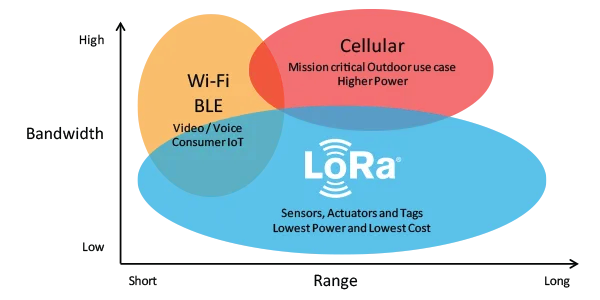
\includegraphics[scale=0.7]{bandwidth-vs-range.png}
\end{figure}
Semtech

Es ist für große Reichweite, kleine Bandbreite und Niedrigenergiekommunikation gemacht. Alles in allem also extrem nützlich für IoT Geräte. Einige Beispiele sind:

\begin{itemize}
	\item Wassersensoren in einer entfernten Umgebung (Grundwasser)
	\item Rauchwarnmelder
	\item Tierbeobachtung
	\item Verbrauchsmessungen bei Endkunden (Gas, Strom)
	\item Wetterstationen die nur ab und zu Informationen übertragen
\end{itemize}

\subsection{LoRa und LoRaWAN}

LoRaWAN ist über LoRa angesiedelt und definiert das Kommunikationsprotokoll und die Systemarchitektur.

Es ist wichtig zu verstehen, dass es möglich ist LoRa ohne LoRaWAN zu benutzen. Andere LoRa basierte Netzwerke sind Helium, The Things Network Disaster.radio und, was wir weiter betrachten werden, Meshtastic.

\subsection{Meshtastic}
Wie im vorherigen Absatz erwähnt, baut Meshtastic auf LoRa auf und schafft ein dezentralisiertes Mesh-Netzwerk.

Es bringt folgende Eigenschaften mit sich:
\begin{itemize}
	\item Verschlüsselte und Textbasierte Kommunikation
	\item Plattformunabhängig
	\begin{itemize}
		\item Computer (unabhänging vom Betriebssystem)
		\item Android (dedizierte Chat-App)
		\item iOS (dedizierte Chat-App)
	\end{itemize}
	\item Dezentralisiert
	\item Geringer Stromverbrauch
	\item Optionales Standort teilen
	\item Open-source
\end{itemize}

Anders als traditionelle Mobilfunknetzwerke, verbindet sich jedes Endnutzergerät mit einem LoRa Radio und alle LoRa Radios, welche Meshtastic nutzen, können Nachrichten, selbst wenn die Radios nicht im gleichen Mesh sind, weiterleiten. Das passiert so lange, bis die Nachricht Ihr Ziel erreicht oder die voreingestellten “Hops” ausgeschöpft werden.

\section{Geräte}

Folgende Geräte haben wir für das Projekt genutzt:

\subsection{Heltec LoRa32 v3}

https://heltec.org/project/wifi-lora-32-v3

max TX power: +21dBm

\begin{figure}
	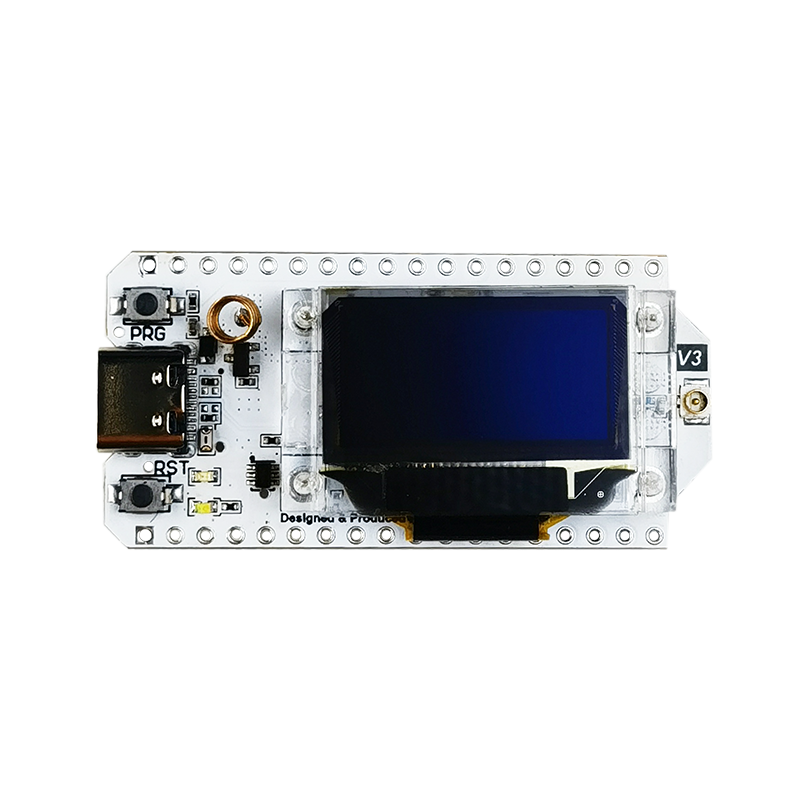
\includegraphics[scale=0.1]{heltec-lora32-v3.png}
\end{figure}

\subsection{LILYGO T-Echo}

https://www.lilygo.cc/products/t-echo


max TX power: +21dBm

\begin{figure}
	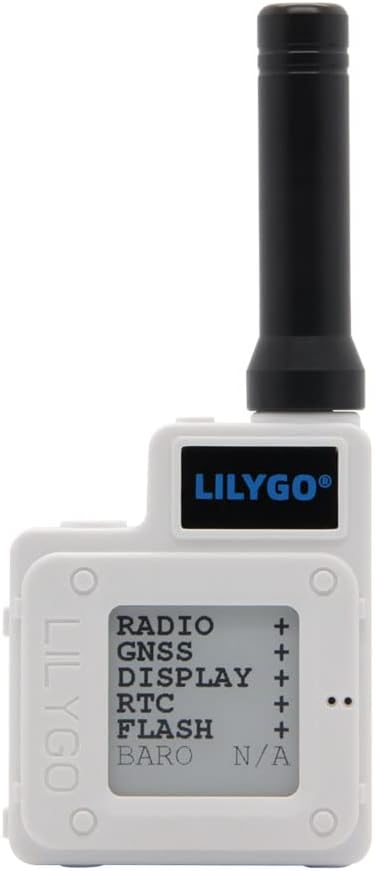
\includegraphics[scale=0.1]{t-echo.jpg}
\end{figure}

\subsection{LILYGO T-Deck}

https://www.lilygo.cc/products/t-deck


max TX power: +21dBm

\begin{figure}
	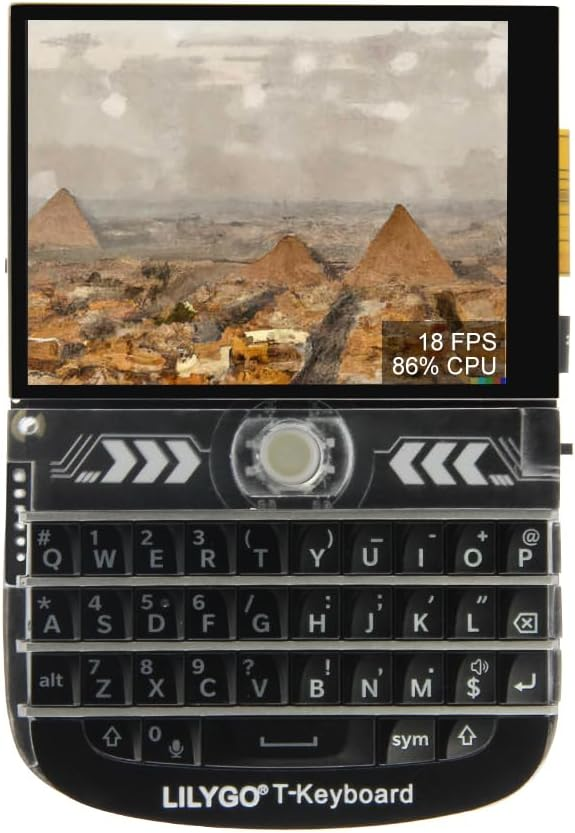
\includegraphics[scale=0.1]{t-deck.jpg}
\end{figure}

\section{Firmware flashen}
Geräte brauchen Firmware

\subsection{Hardware identifizieren oder auswählen}
Achtung!
Vorweg, Geräte nur mit angeschlossener Antenne einschalten! Anderenfalls kann das Gerät sich im schlimmsten Fall selber zerstören.

Meshtastic wird offiziell nur von bestimmten Geräten welche ein LoRa Modul innehaben supportet.

Es ist darauf zu achten, dass jedes Gerät welches im Meshnetz betrieben werden soll auf der gleichen Frequenz arbeitet. Hier gibt es unterschiede!

In deutschland können die freien Frequenzbänder 433 MHz und 868MHz, auf welchen Lora operiert, ohne Lizenzkosten oder Amateurfunklizenz genutzt werden.

Solange WLAN Verbindung zu einem Device nicht notw. ist und Bluetooth ausreicht, sollte ein nRF52 Chip gewählt werden, da diese energieffizienter als ESP32 Chips und einfacher zu flashen sind. Es gibt auch noch Geräte auf Basis des RP2040, diese haben wir allerdings nicht getestet.

Eine Liste mit unterstützer Hardware findet sich hier:

https://meshtastic.org/docs/hardware/devices/

\subsubsection{Serial Treiber für ESP32}
Einen für das eigene Betriebssystem passenden Treiber auf folgender Seite identifizieren, herunterladen und Installieren:

https://meshtastic.org/docs/getting-started/serial-drivers

\subsubsection{Serial Treiber für nRF52}
nRF52 Chips benötigen normalerweise keinen Serial Treiber. Sie benutzen einen UF2 bootloader, welche das Gerät als USB-Stick vom Betriebssystem erkennen lassen.

Auf keinen Fall folgenden USB geräte treiber herunterladen, es sei denn es wird UF2 support benötigt

https://meshtastic.org/docs/getting-started/serial-drivers/nrf52

\subsection{Firmware für ESP32 flashen}
https://meshtastic.org/docs/getting-started/flashing-firmware/esp32/ Da es bei uns auf verschieden PCs probleme gab haben wir zum Flashen unter Linux eine Nix-Flake erstellt, die Python mit den richtigen Paketen installiert und eine kleine Anleitung (auch zum selber Compilieren der Firmware) für esp32 und nRF52 Geräte enthät.

\subsection{Firmware für ESP32 nRF52}
https://meshtastic.org/docs/getting-started/flashing-firmware/nrf52/ Beim diesen Geräten ist es bei uns manchmal vorgekommen, dass das Flashen von Firmware zwar bis zu dem “Drag und Drop”-Schritt funktioniert und dann aber nicht wirklich mit der neuen Version neu startet. Falls das passiert muss man sich mit einer seriellen Konsole mit dem Gerät verbinden und einfach nur einmal Enter drücken, besonders nachdem Factory-Erase. Das steht unter dem Punkt Factory-Erase auch dokumentiert, aber man benötigt nicht zwingend die Meshtastic CLI, sondern lediglich ein Programm wie z. B. minicom unter Linux.

\section{Häufige Probleme - Kommunikation mit Gerät über USB}
\begin{itemize}
	\item Die Gerät-Datei /dev/ttyUSB0 gehört der Nutzergruppe dialout. Damit der Nutzer Schreibrechte erhalten kann, muss er zur Gruppe hinzugefügt werden:
	
	\lstinline{sudo usermod -aG dialout <user-name>}
	
	Der Nutzer muss sich ausloggen und wieder einloggen, damit er in der Gruppe enthalten ist.
	\item Prüfen, ob das Kabel zwischen Computer und Gerät auch wirklich Daten übertragen kann.
	\item USB-C → USB-C funktioniert manchmal nicht. Dies könnte an einem Fehler bei USB-C Power Delivery liegen. Adapter USB-C → USB-A (findet man meist als OTG-Adapter) schafft Abhilfe.
\end{itemize}

\section{Simulation}
TODO LINKS einfügen @goeranh

Die Wartung vieler Meshtastic Nodes für den Zweck des Experimentierens mit der Software bzw. dem Protokoll kommt mit einem größeren Aufwand einher. Dafür kann sich eine Simulation besser eignen, um Resultate ohne Aufwand direkt beobachten zu können.

Mit der Software Meshtasticator ist es möglich, ein Meshtastic Netzwerk zu simulieren. Diese basiert auf zwei vorherigen Simulatoren (lora-network-simulator und LoRaSim) und nutzt unterliegend die Meshtastic Linux Anwendung, weswegen die Verwendung eines Linux Betriebsystems Voraussetzung ist.

Wir haben den Simulator in einer Ubuntu-VM installiert. Einige Pakete mussten installiert werden.
\begin{lstlisting}
	sudo apt install git python3-tk python3-pip \
	python3-venv gpiod libgpiod gpiod libgpiod-dev \
	libgpiod2 libyaml-cpp-dev libbluetooth-dev
\end{lstlisting}

Danach musste man das Meshtasticator und Meshtastic-Firmware Repository herunterladen.

Um die Firmware zu compilieren, benötigt man PlatformIO. Das Tool lässt sich mit dem System Paketmanager wie z.B. apt installieren, häufig bekommt man eine veraltete Version, da die Paketquellen der meisten Betriebsysteme nur langsam aktualisiert werden.

Deshalb empfehlen wir, den Paketmanager von Python zu nutzen:
\begin{lstlisting}
	pip install platformio
\end{lstlisting}

Der Installationspfad liegt in ~/.local/bin, welcher nicht standardmäßig in der Systemvariable PATH enthalten sein kann. Falls der Befehl pio beim Aufruf nicht gefunden wird, reicht es aus, den Installiationspfad zum System-PATH hinzuzufügen:
\begin{lstlisting}
	export PATH="$HOME/.local/bin:$PATH"
\end{lstlisting}

Die Meshtastic Firmware, welche normalerweise für IoT Hardware kompiliert wird, kann auch nativ auf einem Linux Betriebsystem mithilfe von Portduino ausgeführt werden.

Mit Environment-Parameter native baut PlatformIO die Firmware für ein Linux Betriebsystem.
\begin{lstlisting}
	pio run --environment native
\end{lstlisting}

Tipp

Die PlatformIO Extension für VSCode bietet eine praktische GUI, mit der die Befehle ausgeführt werden können.

Das kompilierte Binary befindet sich dann im Ordner \lstinline{firmware/.pio/build/native}.
Damit der Meshtasticator die gewünschten Anordnungen simulieren kann, muss die Binary in den Ordner von Meshtasticator kopiert werden. Bevor die Abhängigkeiten von Meshtasticator installiert werden können, sollte in dem Ordner eine Python-Umgebung aktiviert werden:
\begin{lstlisting}
	python3 -m venv venv
	source venv/bin/activate
\end{lstlisting}
Die Abhängigkeiten können mit \lstinline{pip3 install -r requirements.txt} installiert werden.

\section{Werkzeuge}
\begin{description}


    \item [Programmiersprache]\tab Python
    \item [Open-Source Bibliotheken]\tab Keras \newline \tab \tab Tensorflow
 
 
\end{description}

\section{Was ist Maschinelles Lernen?}
Maschinelles Lernen ist das Fachgebiet, das Computern die Fähigkeit zu lernen verleiht ohne explizit programmiert zu werden
\begin{flushright} - Arthur Samuel 1959  \end{flushright}

\section{Was sind Rekurrente Neurale Netzwerke?}
Placeholder

\subsection{ML-Modell}
$<Grafik>$ \newline
Placeholder
\subsubsection{GRU-Layer}
Why GRU (Vorteile, Nachteile) \newline
Verallgemeinerte(vereinfachte) Grafik (Update Gate, Reset Gate, Current Memory)\newline
Grafik Update Gate\newline
etc.
\subsubsection{LSMT-Layer}
Placeholder
\subsubsection{Dense-Layer}
Placeholder
\subsubsection{Embedding-Layer}
Placeholder
\newpage
\section{Theorie}

\subsection{Link-Budget}

Die Reichweite einer Funkverbindung lässt sich mittel des Link-Budgets (Leistungsübertragungsbilanz) darstellen und gibt die Qualität eines Funk-Übertragungskanals an.
Eines der einfachsten Modelle um ein Linkbudget zu errechnen ist mittels Addition der Sendeleistung (Transmitter Power, Tx), der Empfängerempfindlichkeit (Receiver Power, Rx), des Antennengewinns und der Freiraumdämpfung (Free Space Path Loss, FSPL).

\subsection{Kenngrößen}

Der Spreading Faktor und somit die Reichweite eines Senders sind von den Ausbreitungsbedingungen abhängig.
Die Empfängerempfindlichkeit hängt von Signal-Rausch-Verhältnis (SNR), Rauschfaktor (NF) und Bandbreite (BW) ab.

Die Freiraumdämpfung beeinträchtigt die Reichweite. Durch die Verdopplung der Entfernung nimmt die Freiraumdämpfung um 6 dB zu.
Reflektionen und Brechungen der Funkwellen an Hindernissen und Boden beeinflussen Signalpegel und Reichweite. Im LoRaWAN-Netzwerk befindet sich eine Seite der Funkverbindung in der Regel in Bodennähe.
Hindernisse in der ersten Fresnelzone beeinflussen den Signalpegel auf der Rx-Seite und verkürzen die Reichweite.
SF-Werte und somit die Reichweite eines Senders hängen von den Ausbreitungsbedingungen ab. LoRaWAN erlaubt mittels ADR ein automatisches Netzmanagement und regelt damit die Reichweiten der Sender.

\subsection{dB}

Die Einheit dB (Dezibel) wird im Zusammenhang mit Funkverbindungen verwendet, um die Signalstärke, Dämpfung oder Verstärkung von elektromagnetischen Signalen zu messen. dB ist eine logarithmische Einheit, die das Verhältnis zwischen zwei Größen ausdrückt. In Bezug auf Funkverbindungen sind die beiden häufigsten Anwendungen die Messung der Signalstärke und die Angabe von Dämpfung oder Verstärkung.

1. **Signalstärke in dBm (Dezibel Milliwatt):**

   - dBm misst die absolute Leistung eines Signals im Vergleich zu einem Referenzwert von 1 Milliwatt.
   - Ein positives dBm-Wert zeigt an, dass das Signal stärker ist als 1 Milliwatt, während ein negativer Wert darauf hinweist, dass es schwächer ist.
   - Beispiel: Ein Signal mit -50 dBm ist stärker als ein Signal mit -60 dBm.

2. **Dämpfung und Verstärkung in dB:**
   - dB wird auch verwendet, um die Dämpfung oder Verstärkung von Signalen in einer Leitung oder einem System auszudrücken.
   - Eine positive dB-Angabe deutet auf Verstärkung hin, während eine negative dB-Angabe auf Dämpfung hinweist.
   - Beispiel: Ein Verstärker, der das Signal um 20 dB verstärkt, erhöht die Signalstärke um das 100-fache.

Bei Funkverbindungen wird die Signalstärke oft in dBm gemessen, während Dämpfung oder Verstärkung von Antennen, Kabeln oder Verstärkern in einfachen dB-Angaben ausgedrückt werden. Dies ermöglicht eine präzise und effektive Kommunikation über die Leistung von Funksignalen und die Leistung von Komponenten in drahtlosen Netzwerken.

\subsection{Channelsettings}

|                           |                     |
| ------------------------- | ------------------- |
| Channelsetting            | Long Range / Fast   |
| Alt Channelname           | Long Fast           |
| Data Rate                 | 1.07 kbps (default) |
| Spreading Factor/ Symbols | 11 / 2048           |
| Coding Rate               | 4/5                 |
| Bandwith                  | 250                 |

\subsection{Transceiverwerte}

|                |         |
| -------------- | ------- |
| transmit Power | 21dBm   |
| Antenna gain   | 0dBi  |
| RX sensitivity | -131dBm |
| RX antenna     | 0dBi    |
| Link Budget    | 152dB   |

WiFi LoRa 32 v3 (SX1262 Lora Chip)
P(dBm) = 21dBm
Max Receiving sensitivity = -136dBm@SF12 BW=125KHz

(1)<https://www.semtech.com/design-support/lora-calculator>

\subsection{Maximal mögliche Übertragunsstärke}





\newpage

\section{Discussion}
\section{Summary}
\section{References}
\end{document}
